%!TEX root = project.tex

\chapter*{About this project}
\paragraph{Abstract}
A brief description of what the project is, in about two-hundred and fifty words.

\paragraph{Authors}
Mark Reilly



\chapter{Introduction}

\section{Background}
Millions of people around the world regularly acquire information from weather forecasts for several reasons. Increased availability and access to the internet has allowed for a more suitable way for people to retrieve this information. As a result, weather applications have quickly gained popularity.

The weather is always changing which has a big impact on our daily lives, influencing what we choose to do and how we go about our day. The dynamic nature of the weather means that factors such as temperature and precipitation are constantly changing. Due to this, people are very interested in knowing predicted weather conditions to plan and organise events \cite{WeatherontheGo}. With ever-changing weather, it is crucial for weather stations to provide accurate data to allow for more accurate forecasts. 

The equipment used to collect weather data across Ireland varies depending on the four different types of weather stations. These include Manned Weather Stations which record meteorological elements on an hourly basis using a form, as seen in figure \ref{MetForm}, Automatic Weather Stations record meteorological elements on a minute-by-minute basis, Climatological Stations which record data for climate analysis and meteorological research and lastly Rainfall Stations which record daily and monthly rainfall data. As Ireland experiences extremely distributed rainfall, there are over five hundred of these Rainfall stations in Ireland \cite{MET}.

\begin{figure}[h]
\centering
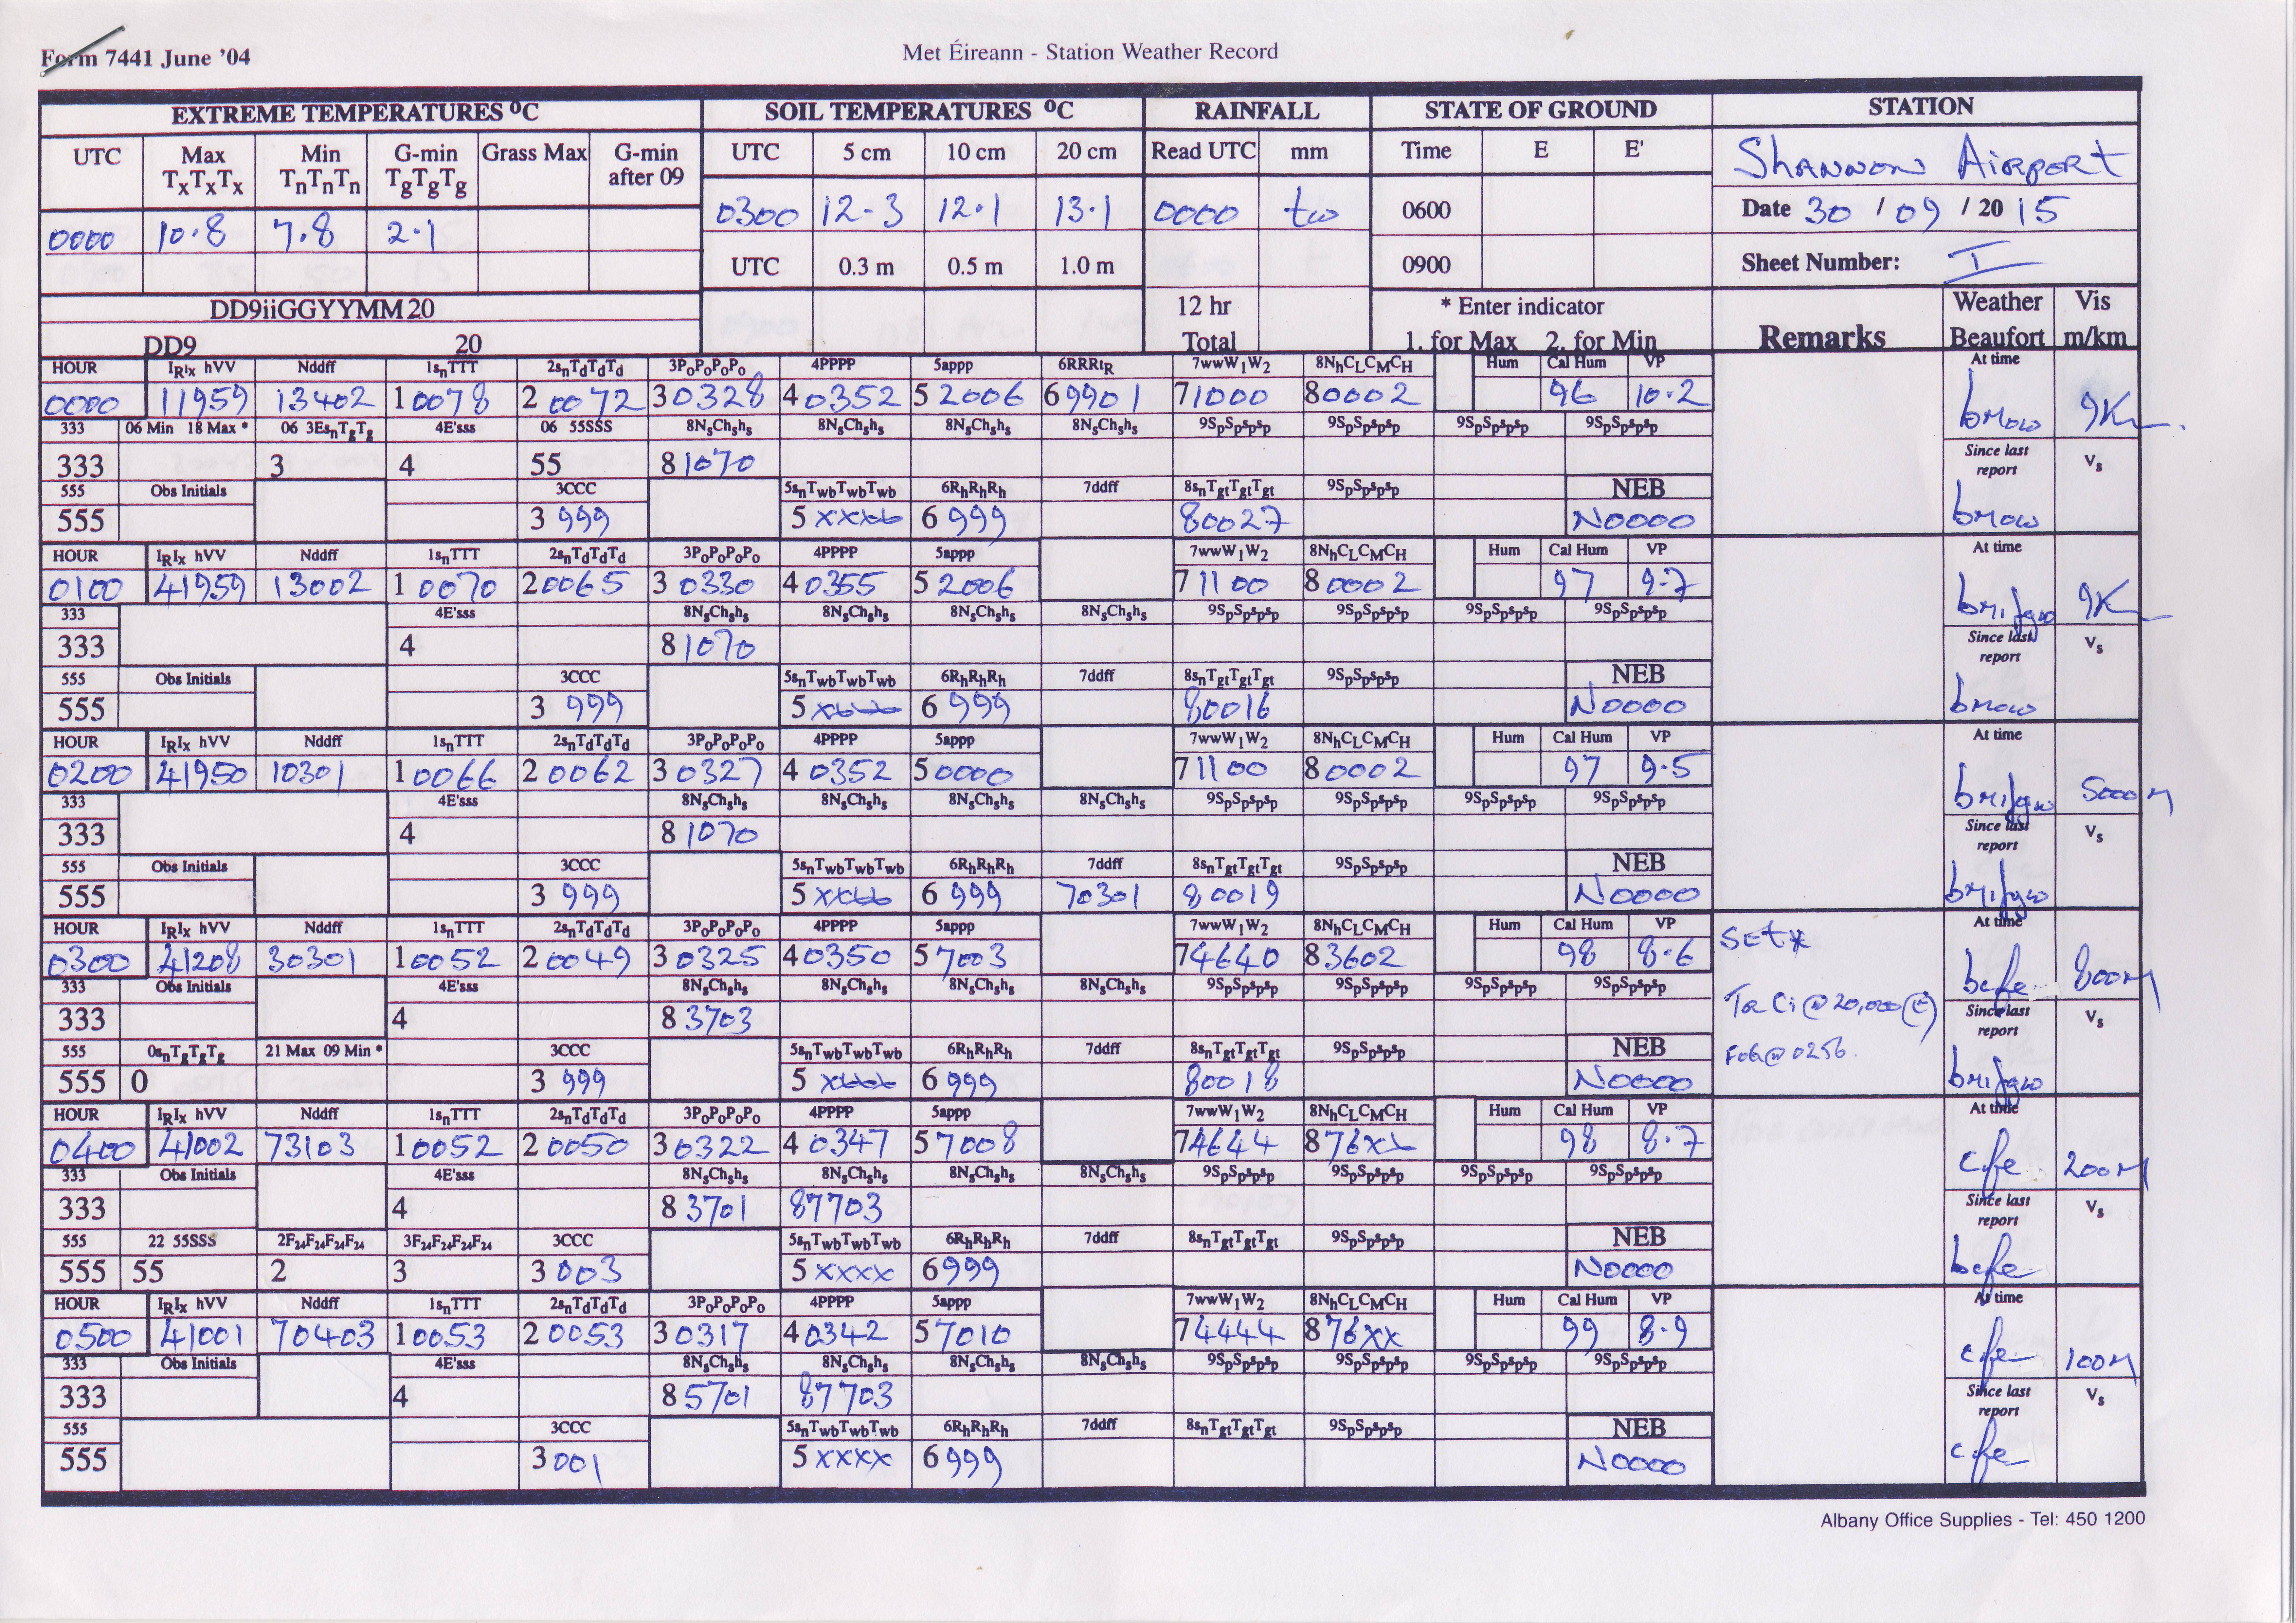
\includegraphics[scale=0.4]{img/MannedWeatherStation.jpg}
\caption{Station weather record form used by meteorological observer at a manned station. }
\label{MetForm}
\end{figure}
Of note, there are several weather instruments used to gather data such as thermometers, anemometers, rain gauges, hygrometers etc. However, since this project is focusing on the prediction of temperature and rainfall values, only thermometers and rain gauges will be discussed.

Thermometers measure the high and low outdoor temperature in degrees Celsius or Fahrenheit. Nowadays, electronic maximum-minimum temperature sensor systems are used, see figure \ref{Thermometer} whereas in the 1800s liquid in glass thermometers were utilised.\cite{WeatherInstruments}

\begin{figure}[h]
\centering
\includegraphics[scale=0.2]{img/MaxMinThermometer.jpg}
\caption{Electronic Thermometer used to collect temperature data.}
\label{Thermometer}
\end{figure}

Rain gauges are used to measure the amount of rainfall. There are two types of rain gauges, the storage rain gauge and the tipping bucket rain gauge, see figure \ref{Gauge}. The latter is more widely used due to it being more automated with less maintenance.\cite{RainGauge}

\begin{figure}[h]
\centering
\includegraphics[scale=0.2]{img/storageRainGauge.jpg}
\includegraphics[scale=0.2]{img/tippingBucketGauge.jpg}
\caption{The Storage Rain Gauge and The Tipping Bucket Rain Gauge}
\label{Gauge}
\end{figure}

\section{Project Objectives}
There are currently multiple weather applications available that give a wide variety of information on weather forecast. However, most of these applications depend solely on application programming interface (API) data and very few integrate both API and machine learning data into one application. Therefore, the aim of this project is to develop a full-stack weather application that uses both API data and machine learning to predict certain weather conditions. 

\section{Web Application Development}
A web application (WA) is a computer program that utilises both web browsers and web technology to perform tasks over the internet. WA development is the creation of application programs that reside on servers and are delivered to the user's device over the internet \cite{WebAppDef}.

WA's use a combination of server-side scripts (Django) to handle the storage and retrieval of dataand client-side scripts (ReactJS) to display that data to users \cite{WebApp}. Client-side refers to an application running on a web browser. Client-side programming typically utilizes HTML, CSS and JavaScript combined with a frontend framework such as ReactJS. Server-side programming powers the client-side programming and is used to create scripts that enable the web application to have various features. Server-side programming has many different coding languages such as Python, Ruby, Java \cite{WebAppDef}.

Data is exchanged over the network using HyperText Transfer Protocol (HTTP). An advantage of this approach is that the user's do not depend on any specific operating system or hardware configuration. Hence, WA's are cross-platform software. They vary in functionality and design but are set up to serve the same purpose, which is to provide the user with features and accessibility to information.

The application developed would provide consistent weather forecast updates and also be a significant improvement compared with similar websites by allowing access to more premium features from any location. 

\section{History of Machine Learning}
Machine Learning (ML) is a subset of artificial intelligence where computers can self-learn from data and information. ML algorithms automatically build a model of sample data also known as — "training data" — to make decisions without being specifically programmed to make those decisions \cite{MLAlgorithms}.

The first computer learning program was written by Arthur Samuel in 1952. He designed a program that was a game of checkers which used a minimax strategy to decide on the next move. After playing more games it studied which moves made up winning scenarios and incorporated these into the program. The minimax strategy later became known as the "Minimax Algorithm" \cite{MiniMax}.

A few years later, in 1957, Frank Rosenblatt designed "The Perceptron" which was the first neural network for computers. It was designed with the efforts of Donald Hebb's model of brain cell interaction and Arthur Samuel's ML knowledge to simulate the thought process of the brain. In the years 1967 to the early 2000s, there were many developments in the ML area such as the "nearest neighbor" algorithm. It allowed computers to use basic pattern recognition, the concept of Explanation Based Learning in which a computer analyses data and creates a rule to discard unimportant data. ML shifted from a knowledge-driven approach to a data-driven approach, creating programs that could analyze large amounts of data and learn from the results \cite{MLAlgorithmsHistory}.

The late 2000s was when ML started to gain recognition outside of the computer world due to ML featuring in more widely used devices such as The Microsoft Kinect. The Microsoft Kinect allowed users to interact using gestures, Facial Recognition being used in mobile devices for security purposes and speech recognition which is done by a deep learning technique called Long Short-Term Memory (LSTM) is used in Apples Siri \cite{MLAlgorithmsHistory}.

Present-day ML is also responsible for some of the most important technological advances, such as the emerging self-driving car industry and chat assisted robots. ML models have become increasingly more efficient in continuously learning from training data which in turn makes them more accurate with increased data to learn from. Ml models can be used for a variety of reasons from predicting the weather to predicting stock prices.
\newpage
\section{Scope of Project}
\begin{enumerate}
\item User-friendly web application.
\item Fully functional weather predictions.
\item Consistent forecasts.
\item Login and Register system.
\item About page providing information on the application.
\item Visually pleasing design.
\item Similar features to competitor applications.
\end{enumerate}

\chapter{Context}
\section{Project Objectives}
In this section, I will outline the key objectives for this project.
\begin{itemize}
    \item To provide an aesthetically pleasing UI.
    \item To provide a reliable weather application.
    \item To provide REST API to weather forecasts.
    \item To provide a scalable application.
    \item To provide user security with storage of personal information.
    \item To provide low load times when retrieving information.
\end{itemize}

\section{Weather Application}
A weather application is increasingly important in today's modern world, with easier access to online resources and access from nearly any location with a mobile phone signal it has led to a significant rise in numbers using web applications. Gone are the days of waiting for specific times in the day to tune in for the daily/weekly weather reports on the radio/TV. The use of weather applications that are supported on any device with a browser has led to a revolution in the way we get the latest weather. In this chapter, I will discuss the advantages, disadvantages, and overall impact of weather applications.

\section{Advantages Weather Applications}
In this section, I will discuss the advantages of weather applications.

\subsection{Reliability}
There are many advantages to weather applications which I will discuss in this section, the most noteworthy of those is reliability. Taking into consideration the advancements in weather data collection in recent years has led to more widely available weather information, which in turn provides weather applications with more reliable forecasts. Users of these apps will now see what the weather will be like in the coming week; a weather forecast will provide a very accurate picture of what to expect. A seven-day forecast can predict the weather about 80\% of the time, whereas a five-day forecast can predict the weather about 90\% of the time. \cite{weatherReliability}. 

\subsection{Competitors}

The rise in various weather applications over the years means that each application is trying to add new features to stand out from the crowd. The customer benefits from this competitive nature within these businesses allowing them to have more choice in which application they use. 
\subsection{Convenience}
Frequent users of weather applications now only have to open an application on their smart device to gain access to tonnes of weather information. The user can now plan their day/week in advance at any moment rather than having to wait for a certain time in the day when the weather report would be on a radio or TV. The benefit of this convenience is that the user gains more information at the touch of a button and they save time looking for weather forecasts when it is all in one area.

\section{Disadvantages Weather Applications}
In this section, I will discuss the disadvantages of weather applications.

\subsection{Inaccurate weather predictions}

Weather predictions are never 100\% and it is almost impossible to predict the future with certainty. Even if you have a great process in place and forecasting experts on your payroll, your forecasts will never be spot on. Some applications will have a high level of volatility depending on which weather data provider they are using. The main drawback of forecasts is that they are almost always inaccurate - which leads to a dissatisfied customer.

\subsection{Security}

Storing details in a digital environment is a lot less secure than storing those same details in a non-digital environment. The reason for this is due to that data being stored on a server that is vulnerable to attacks such as SQL Injection - When a perpetrator manipulates a backend database with malicious SQL code, information is revealed. Consequences include the following: unauthorized lists can be viewed, tables can be deleted, and unauthorized administrative functions can be performed \cite{sqlInjection}. Gaining access to such a database on a weather application may hold users' personal details, card details, and address details.

\subsection{Internet Reliance}

An internet connection is a must with the web application for it to load any data. There will be a lack of updated information if internet connectivity is lost during browsing. Web applications cannot run without the internet which makes them redundant in areas with little to no internet. 

\section{Overall Effect Weather Applications}

The overall effect of weather applications has had a resounding impact on the way customers plan ahead. The reliability and convenience of everyday weather applications to the mass population of the world have led to more advantages than disadvantages in my personal opinion.
\newpage
\section{Outline of each chapter}
Below I will outline the chapters that my Dissertation is broken up into and give a brief outline of each one.

\subsection{Introduction}
In Chapter 1, I will give an outline of the overall project and then proceed to discuss the background of the weather. I will then discuss web application development and the history of machine learning to give the reader an understanding of the project.

\subsection{Context}
In Chapter 2, I will discuss the context of my project and how weather applications have changed how we view the weather. I will research the advantages and disadvantages of weather applications for users.

\subsection{Methodology}
In Chapter 3, I will discuss the methodology I followed and how it affected my project and productivity. I will also discuss how I planned to complete the project and discuss the methodologies I utilized in the process. I will discuss why I chose these methodologies and give the reader an insight into how this application was developed. 

\subsection{Technology Review}
In Chapter 4, I will discuss the technical aspects of this project and discuss how each technology impacted the development cycle of this project. I will also discuss why each technology was implemented over other available technologies. I will discuss the three main technologies chosen for this project in detail and how I utilized each of them to create a Full Stack Weather Application. 

\subsection{System Design}
In Chapter 5, I will explain the architecture and design of the project. I will use graphs, diagrams, and screenshots to help explain the rationale of how the application is designed and how it will operate when deployed. I will discuss various main functions in the code to give an overview of how the main features of the application work.

\subsection{System Evaluation}
In Chapter 6, I will test the software and evaluate whether it is robust and meets all the objectives I have specified. I will highlight any limitations in the approach used and the technologies used.

\subsection{Conclusion}
In Chapter 7, I will outline what I have learned from this project and highlight any findings from the system evaluation chapter. I will discuss the impact the project had on my skills as a software developer and how working remotely during a global pandemic impacted the development stage of the project. I will also summarise what I would do differently if I was to do this project again.

\section{Github Structure}

The \href{https://github.com/MarkReillyGMIT/AppliedProject}{Github} resource URL can be found by clicking \href{https://github.com/MarkReillyGMIT/AppliedProject}{Here}. The git repository contains four folders: Dissertation, ReadMeFiles, backend, and front-end. The Dissertation folder contains all files related to the development of the dissertation document. The ReadMeFiles folder contains all images that will be displayed on the README. The backend folder contains all the related code for the Django backend and neural network computation. The front-end folder contains all the related code for the ReactJS front-end. There is a requirements.txt file that has all the required libraries necessary for the project to run. The README.md file will contain a brief description of the project and how to run the project. The gitignore file is a text file that tells Git which files or folders to ignore in a project. 


\chapter{Methodology}

\section{Overview of Methodology}

In this project, I took an agile approach to development using the Agile Methodology. I used sprints to manage my work during the development life-cycle.

\section{Agile}
In this section, I will discuss the Agile Methodology which was utilised in the development process of this application.

\subsection{What is Agile?}
Agile methodology is a practice that promotes continuous iteration of development and testing throughout the software development life cycle of the project. In the Agile model, both development and testing activities are concurrent, unlike the Waterfall model\cite{Agile}. Agile is a term used to describe software development approaches that employ continual planning, learning, improvement, team collaboration, evolutionary development, and early delivery. It encourages flexible responses to change \cite{Agile}. There are many different agile methodologies to chose from such as Kanban, Scrum, Extreme Programming (XP), Crystal, Dynamic Systems Development Method (DSDM). For the purpose of this project, I will be using Scrum. 

\begin{figure}[h]
\centering
\includegraphics[scale=0.4]{img/agile-development-chart.png}
\caption{Agile Development Lifecycle}
\label{Agile}
\end{figure}


\newpage

\section{What is Scrum?}
SCRUM is an agile development method that concentrates specifically on how to manage tasks within a team-based development environment. Basically, Scrum is derived from an activity that occurs during a rugby match \cite{Agile}. Since SCRUM is mainly used for team projects I had to adapt it to suit my needs. It consists of three roles which are as follows:

\begin{itemize}
    \item Scrum Master - responsible for setting up the sprint meetings and removing challenges to progress \cite{Agile}.
    \item Product Owner -  creates the product backlog and is responsible for the delivery of the product. Sharing the vision for the product with the team \cite{Agile}.
    \item Scrum Team - manages its work and organizes its work to finish the sprint of cycle \cite{Agile}.
\end{itemize}

\begin{figure}[h]
\centering
\includegraphics[scale=0.4]{img/scrum.png}
\caption{Scrum Development}
\label{Scrum}
\end{figure}

\subsection{Adapting Scrum}
In this section, I will discuss how I adapted the scrum methodology into my individual project. 

During the project, I dedicated time to planning the project weeks in advance. Using a Gantt Chart to plan and keep track of weekly tasks and milestones. The Gantt chart software that I used was on \href{https://app.clickup.com}{Clickup} which was provided for free. It allowed for the adding of tasks and milestones which then could be marked as "Open", "Closed", "Completed". There were also email notifications available that provided an update on tasks that were soon to be overdue. There was a lack of free Gantt Chart software available online which made it difficult and time-consuming to find a good standard free version. See Figure \ref{Gantt}.

\begin{figure}[h]
\centering
\includegraphics[scale=0.4]{img/GanttChart.PNG}
\caption{Gantt Chart}
\label{Gantt}
\end{figure}

\subsection{Planning Sprints}

I planned my sprints using the tasks on the Gantt chart, each task was added with a certain amount of time depending on the difficulty of the task. Setting reasonable and attainable goals for each week. See Figure \ref{Gantt} to view the variable time lengths that were given to each task.

\subsection{Conduct Weekly Scrums}

I scheduled a time each week to review my previous week's work to identify any successes and pitfalls \cite{Scrum}. I had to then act as the scrum master to find solutions to any problems I may have encountered that week. Referring to my Gantt chart for a visual idea of where I could find the time to fix the problems encountered.

\subsection{Review your sprint}
At the end of the sprint, I would consider the downsides and upsides of the process. Taking into consideration how closely the results align with the overall vision for the project \cite{Scrum}. 

\section{Test Driven Development}
In this section, I will discuss Test-Driven Development (TDD), what it is and how I incorporated it into the development process.

\subsection{What is Test Driven Development}
TDD is a software development approach in which test cases are developed to specify and validate what the code will do. In simple terms, test cases for each functionality are created and tested first and if the test fails then the new code is written in order to pass the test and make code simple and bug-free \cite{TDD}. See Figure \ref{TDD}.

\begin{figure}[h]
\centering
\includegraphics[scale=0.5]{img/TDD.png}
\caption{Test Driven Development Cycle}
\label{TDD}
\end{figure}

\subsection{How I incorporated TDD into the project}
I applied TDD into the project by writing tests into various parts of the code as I was in the development phase. I wrote print-out statements to the command line for the backend to analyze the values that were being sent. For the front-end, I wrote tests that could be viewed using the inspect element to analyze the correct data that was being displayed on the web application. I continued to write enough code to make the test pass and then refactored it, repeating this process for each test. 

\section{Git Version Control}
In this section, I will discuss version control and how I managed to develop the project by using Github and Git. I used \href{https://github.com/MarkReillyGMIT/AppliedProject}{Github} to manage all the code and files for the project while using Git to commit any new/updated code to the Github repository. Using Github had many beneficial factors such as file management, project management tools, and online file storage. 

In the project section on Github, I utilized the Kanban board which helped with managing any issues I was facing and keeping track of each issue. Github also allows for multiple branches to be created which can be helpful for team projects but in this individual project, I decided to only use the Master branch as I was the only person committing to this project.

Git version control allowed for the tracking of files and any changes made to each file. This really helped when needing to revert back to a previously working version of the project. 

\section{Time Management}
In this section, I will discuss how I manage my time during the development phase of the project and the issues I faced throughout.

\subsection{Management of Several Projects}
I was able to manage multiple projects at a time by using the Gantt chart to set out my weekly task and assigning different days to various modules. The tasks sometimes became tough to complete on time as the workload of other modules was heavy at certain times of the year. 

\subsection{Issues Faced}
I faced many issues throughout the project as the workload was immense. Here a list of the top issues faced:

\begin{itemize}
    \item Difficulty in finding a quiet work environment due to college being closed.
    \item Standard of projects was dropped due to heavy workload.
    \item Slow internet due to location.
    \item Covid-19 illness.
    \item Procrastination. 
\end{itemize}
\newpage


\chapter{Technology Review}
\section{Overview}
In this chapter, I will discuss the technologies used in this project at a conceptual level. I will explain why I used these technologies, how they were implemented and utilized to allow for a fully functional weather application. I will also review each technology utilized and show how each technology gave a different functionality in reaching the end vision of the project. 

\section{ReactJS}
In this section, I will discuss ReactJS, what it is and the features it provides.

\begin{figure}[h]
\centering
\includegraphics[scale=0.2]{img/ReactJS.png}
\caption{ReactJS}
\label{React}
\end{figure}

\subsection{About ReactJS}
ReactJS is a JavaScript library that is deployed to develop reusable user interface (UI) components. ReactJS enables the development of large and complex web-based applications or mobile applications which can change their data without subsequent page refreshes. ReactJS abstracts the Document Object Model (DOM), offering a simple, performing and robust application development experience \cite{aggarwal2018modern}. ReactJS is only concerned with state management and rendering that state to the DOM. Using ReactJS usually requires additional libraries for other functions such as routing.


\subsection{Features of ReactJS}
\paragraph{A) Lightweight DOM For Optimum Performance.}
ReactJS creates a much more efficient and lightweight DOM. In the majority of other web development frameworks, the browser DOM is directly communicated with which results in the entire DOM tree being changed for every piece of data or event happening on each page \cite{aggarwal2018modern}. This adversely affects the performance when there are large amounts of data being processed. 
On the other hand, ReactJS has for every DOM object there is a "virtual DOM object", which is a lightweight copy. The virtual DOM object has the same properties as a real DOM object but it does not have the power to change what is on the screen. Manipulating the DOM is slow but manipulating the virtual DOM is faster as nothing gets written to screen. This results in fast and robust performance of the application.

\paragraph{B) Easy Learning Curve.}
The difference between ReactJS and other JavaScript libraries is that ReactJS enables one to quickly get comfortable with the framework. The learning curve is extremely easy and one gets along without many complications \cite{aggarwal2018modern}. The framework itself is relatively simple to learn unlike other frameworks where you have to learn the concepts of the framework \cite{aggarwal2018modern, islam2017reactjs}. 

\paragraph{C) JSX.}
JSX is a JavaScript Extension Syntax used in ReactJS to easily write HTML and JavaScript together. It is not mandatory to use JSX while developing a ReactJS application but it is recommended because of how easy development is made using it. I have used JSX in this project. See below for an example of JSX code and see figure \ref{JSX} for the output of the below code. Only few lines at the top are used to import some ReactJS APIs. Except for if-else sentences, we wrap every JavaScript expression in curly braces to embed it in JSX. However, conditional statements can be used. Below is the example where conditional expressing is embedded in JSX \cite{JSX}.

\begin{minted}{javascript}
import React from 'react';
import ReactDOM from 'react-dom';
 
let i = 1;
 
const element = <h1>{ (i == 1) ? 'Hello World!' : 'False!' } <h1>;
  
ReactDOM.render(
    element,
    document.getElementById("root")
);

\end{minted}
\begin{figure}[h]
\centering
\includegraphics[scale=0.3]{img/JSX.png}
\caption{JSX}
\label{JSX}
\end{figure}

\paragraph{D) One Way Data Binding}
One way data binding means that when designing an application often the child components are nested within the parent components. This helps components be simple and predictable. One way data flow ensures that data flows throughout the application in a single direction to allow for more control between the states and models in the application \cite{laydeveloping}. If a change is made on the upstream data, the components using that data downstream will re-render and display those changes.  

\begin{figure}[h]
\centering
\includegraphics[scale=0.3]{img/OneWayDataFlow.png}
\caption{One Way Data Binding}
\label{OneWayDataFlow}
\end{figure}
\newpage

\section{Comparing ReactJS and AngularJS}
In this section, I will compare ReactJS and AngularJS to show the differences between each framework and the attributes that influenced my decision into picking ReactJS. 

\begin{center}
\begin{table}[h]
 \begin{tabular}{ |p{3cm}||p{4cm}|p{4cm}|  }
 \hline
 \multicolumn{3}{|c|}{AngularJS V ReactJS} \\
 \hline
 Attribute & AngularJS & ReactJS \\ [0.7ex] 
 \hline
 DOM & Regular DOM & Virtual DOM  \\
 \hline
 Learning Curve & High & Low  \\
 \hline
 Packaging & Weak & Strong  \\
 \hline
 Abstraction & Weak & Strong \\
 \hline
 Rendering & Client side & Server side \\
 \hline
 Community & Large & Growing \\
 \hline
 Binding & Two way & Uni-Directional  \\ [1ex] 
 \hline
\end{tabular}
\caption{\label{tab:comparing}Comparing ReactJS and AngularJS \cite{kumar2016comparative} }
\end{table}
\end{center}

\subsection{Comparison Conclusion}
The stand-out differences that influenced my decision in picking ReactJS were the learning curve, packaging, debugging, and the virtual DOM. I wanted a relatively easy learning curve as all the technologies were new to me in this project. When researching I learned that there are many packages and libraries compatible with ReactJS.

\section{Django}
In this section I will discuss Django, what it is, the features it provides, and compared it with the rails framework.


\begin{figure}[h]
\centering
\includegraphics[scale=0.3]{img/django.png}
\caption{Django Logo}
\label{Django}
\end{figure}

\subsection{About Django}
Django is a high-level open-source Python web framework that encourages rapid agile development. It was released publicly in July 2005. In June 2008, it was announced that a newly formed Django Software Foundation (DSF) would maintain Django for the future \cite{vainikka2018full}. Since Django is a web application framework based on Python, you need Python to use it. Django officially supports PostgreSQL, MySQL, Oracle, and SQLite databases which influenced my decision in choosing Django, which I will later discuss below \cite{ghimire2020comparative}.

Django also loosely applies the Model-View-Controller (MVC) architecture \cite{ghimire2020comparative} but is mainly a Model-Template-View (MTV) framework. When creating a Django application you are given the following files: models.py, views.py, urls.py, and an HTML template. Models.py is the part of the web app which acts as a mediator between the website interface and the database, it contains the business logic in Django Architecture. Views.py contains the UI logic in the Django architecture. Views.py is the UI of the web application in Django but I will be using ReactJS instead for this project. The role of the urls.py is to control which view is shown on the browser, essentially routing for the application.

\subsection{Features of Django}
\label{marker}
\paragraph{A) Security}
 Security \cite{ghimire2020comparative}- This plays an important role in managing and maintaining the end user's information. Its user authentication system provides a secure way to manage user accounts and passwords. There are many types of threats and vulnerabilities on the web, which can target unsecured web applications. Django covers many security issues:
\begin{itemize}
    \item Cross-site scripting (XSS)
    \item SQL injection
    \item Clickjacking
    \item Host header validation
    \item SSL/HTTPS
    \item Cross-site request forgery protection (CSRF)
\end{itemize}


\paragraph{B) Scalability}
Django is an extremely scalable framework that makes it suitable for high-load projects. When working with a variety of technologies such as ReactJS, PostgreSQL, etc., maintaining loading time and performance could be very challenging. It can process data in a limited time, therefore, reducing the loading time. Django ensures error-free output irrespective of the complexity of coding. 

\paragraph{C) Flexibility}

Django web framework includes many features which allow for it to be versatile in functioning independently. It works on using the MVC architecture and logical project structure which may reduce its flexibility. However, it benefits developers by providing solid coding, allowing it to be used with various other technologies. Inbuilt supports are thoroughly tested since it is an open-source framework.

\paragraph{D) Developer Support}
Compared with other open source technologies, it offers the best documentation in the market. Developers do not need to spend hours reading the code to know how the implementation works. Can easily search for any desired function with ease. There are many basic tutorials on the main website for beginners. Following the instructions in the tutorial one can quickly have an application running in no time. 

\section{Comparing Django and Rails}
n this section I will compare Django and Rails to show the differences between each framework and the attributes that influenced my decision into picking Django. 

\subsection{Brief Overview of Flask}
Flask is a Python micro-framework designed to create web applications in a short time. The framework can be used for just the backend as well as the front-end if need be. Only implements core functionality giving developers the flexibility to add the feature as required during the implementation phase \cite{ghimire2020comparative}.

\subsection{Popularity}
Django and flask are python's most popular frameworks, this one of the reasons why I decided to compare the two frameworks. I decided to compare the popularity of the two using their Github stats and active projects. 

At the time of writing this document, Django has 57,200 stars, it's been forked 24,500 times and currently has 2,300 watchers on Github. See Figure \ref{DjangoStats}.

\begin{figure}[h]
\centering
\includegraphics[scale=0.4]{img/djangoStats.PNG}
\caption{Django Stats on Github}
\label{DjangoStats}
\end{figure}

However, Flask has 54,800 stars, its been forked 14,300 times, and currently has 2,300 watchers on Github. See Figure \ref{FlaskStats}.

\begin{figure}[h]
\centering
\includegraphics[scale=0.4]{img/flaskStats.PNG}
\caption{Flask Stats on Github}
\label{FlaskStats}
\end{figure}

Both frameworks have been used in quite many active projects. The well-known projects powered by Django include Pinterest, Eventbrite, and Instagram. Projects that are using Flask include Twilio, Netflix, and Uber. Django is often the main framework used in the applications whereas Flask is often used just for APIs (Pinterest and Twilio).

\subsection{Security}
Django has built-in security against various attack methods such as CSRF, XSS, and SQL injection as mention in Section \ref{marker}. Django team proactively discloses and patches identified security threats \cite{FlaskVDjango}. However, Flask has a much narrower code base leaving less surface area for a strike to happen \cite{FlaskVDjango}. 

\subsection{Packages}
Django is full of built-in packages. This means you will likely find a package to build and run on your application with less effort. Flask, on the other hand, is minimalistic and has no restrictions, meaning developers can design and implement exactly what they want using external libraries. Allowing Flask to be flexible and scalable when programming your project. 
\subsection{Comparison Conclusion}
The stand-out difference that influenced my decision in picking Django over Flask was how popular it was, meaning there would be more documentation and real-world examples. The other reason was security as I felt it was necessary to have a high level of security when the application is collecting end user's names and passwords.

\section{Database}
In this section, I will discuss the database used in my project, what it is, the features it provides, and compare it with another database.

\begin{figure}[h]
\centering
\includegraphics[scale=0.4]{img/postgreSQL.jpg}
\caption{PostgreSQL Logo}
\label{PostgreSQL}
\end{figure}

\subsection{About PostgreSQL}
PostgreSQL is a free open-source object-relational database management system. It extends the SQL language combined with many features that safely store and scale the most complicated data workloads \cite{vainikka2018full}. Postgre originated back in 1986 as part of the Postgres project at the University of Berkeley but then ten years later changed its name to PostgreSQL to reflect its SQL support. PostgreSQL includes a number of features aimed at assisting developers in the development of applications, administrators in the protection of data integrity and the creation of fault-tolerant environments, and you in the management of your data, regardless of its size \cite{PostgreSQL}. PostgreSQL has earned a strong reputation for its proven architecture, reliability, data integrity, robust feature set, extensibility, and the dedication of the open source community behind the software to consistently deliver performing and innovative solutions \cite{PostgreSQL}. PostgreSQL features transaction with  Atomicity, Consistency, Isolation, Durability (ACID) properties which I will discuss in further detail in the below section. PostgreSQL been ACID compliant since 2001 .

\subsection{Features of PostgreSQL}

\paragraph{A) Ease of Use}
With its complete stack of RDBMS database features and capabilities, PostgreSQL is an easy-to-use database that can manage both structured and unstructured data. On Linux-type settings, yum or source code from the PostgreSQL website can be used to conveniently install the database. When you install from source code, you have a lot of power over the installation. 

\paragraph{B) Supported Data Types}
PostgreSQL supports not only standard SQL data types (such as Numeric, Strings, Date, Decimal, and so on), but also unstructured data types (such as JSON, XML, and HSTORE), as well as network data types, bit strings, and so on \cite{PostgreFeatures}. 

PostgreSQL is distinguished by its support for a broader variety of data types for storing and processing spatial data, including ARRAYs, NETWORK types, and Geometric data types (including specialized spatial data functions). Here is a list of data types that are supported. An additional module called PostGIS, which is an open-source extension, provides support for spatial data types and functions \cite{PostgreFeatures}.

\paragraph{C) Storage}
Any database's ability to store data is crucial. PostgreSQL offers a variety of data storage options. Storing data entails putting physical database objects on a disk, such as Tables and Indexes \cite{PostgreFeatures}.

Tablespaces are a popular storage function in PostgreSQL that can hold physical objects such as Tables, Indexes, and Materialized Views. Tablespaces allow objects to be clustered and stored across several physical locations, allowing for more efficient I/O distribution. PostgreSQL currently does not support pluggable storage engines, although this is planned to change in the future \cite{PostgreFeatures}.

\paragraph{D) Security}
Database protection is critical in preventing unauthorized access to data. Secured access is enforced in the database at different levels, including the object and relation levels \cite{PostgreFeatures}.

GRANT commands in PostgreSQL grant access to database objects and data based on ROLES and PRIVILEGES. Connection authentication is handled in a more straightforward manner, with a pg hba.conf authentication file containing a list of IP addresses, as well as the username and access form. This is much more dependable and straightforward \cite{PostgreFeatures}.
    
\section{Architecture}
This section will describe the architecture of the application.

\subsection{REpresentational State Transfer (REST)}
REST, or REpresentational State Transfer, is an architectural style for establishing standards between web-based computer systems, allowing them to interact more easily. REST-compliant systems, also known as RESTful systems, are distinguished by their statelessness and separation of client and server issues \cite{RESTAbout}. REST defines 6 architectural constraints which make any web service – a true RESTful API \cite{REST}.

\paragraph{1) Uniform Interface}
You MUST determine API interfaces for resources within the framework that are exposed to API consumers and obey them diligently, as the constraint name implies. A resource in the system should only have one logical URI, which should allow for the retrieval of related or additional data. It's often easier to use a web page as a synonym for a resource \cite{REST}.

Throughout the scheme, resource representations should adhere to strict guidelines such as naming conventions, connection formats, and data formats (XML or/and JSON). All resources should be accessible using a common method, such as HTTP GET, and updated using that technique.

\paragraph{2) Client-server}
This constraint simply implies that the client application and the server application must be able to develop independently of one another. Only resource URIs should be known by the client. This is now common practice in web production, so you won't have to do something special \cite{REST}.

\paragraph{3) Stateless}
Any client-server interaction should be stateless. The server will not keep track of the client's most recent HTTP request. Every request will be treated as though it were a new one. There is no session, and there is no past.

If the client application is required to be a stateful application for the end-user, where the user logs in once and only performs other approved operations, then each client request should provide all of the information required to service the request, including authentication and authorization details \cite{REST}.
\paragraph{4) Cacheable}
The importance of caching data and responses is critical wherever they are applicable/possible. Since the load is reduced, caching improves client-side performance and gives a server more scalability options. When caching is used in REST, it must be applied to resources that are cacheable, and these resources must declare themselves cacheable. Caching can be done on the server or on the client \cite{REST}.
\paragraph{5) Layered system}
REST enables you to use a layered system architecture, such as deploying APIs on server A, storing data on server B, and authenticating requests on server C. Normally, a client cannot say if it is linked directly to the end server or via an intermediary \cite{REST}.
\paragraph{6) Code on demand}
This restriction, on the other hand, is optional. The majority of the time, you'll be submitting static resource representations in the form of XML or JSON. However, if you need to return executable code to support a part of your application, you can do so. For example, clients can call your API to get UI widget rendering code \cite{REST}.


\section{APIs}

This section will describe the various APIs in the application that were used to power different features. Each API will be discussed in detail below.

\subsection{Open Weather}
The Open Weather API allows for free API calls on certain data. It is an integral part of the project as this is were the majority of the weather data came from to support the displaying of this data on the front-end. They provide essential weather parameters such as temperature, precipitation, probability of precipitation, humidity, feels like, pressure, cloudiness, wind, etc. 
\subsection{React Leaflet}
The \href{https://react-leaflet.js.org/docs/start-introduction}{React Leaflet} API allow for the feature of a interactive map to be displayed. React Leaflet allowed for bindings between React and Leaflet. \href{https://leafletjs.com/}{Leaflet} was created with ease of use, efficiency, and functionality in mind. It runs smoothly on all major desktop and mobile platforms, can be extended with a large number of plugins, and has an elegant, well-documented API as well as easy, readable source code.

\section{Libraries}
This section will describe the various React and JavaScript libraries used in the development process of the application. These libraries allowed for enhanced features and enjoyment for the end user's. 

\subsection{Scikit-Learn}
Scikit-learn is perhaps Python's most useful machine learning library. Classification, regression, clustering, and dimensionality reduction are only a few of the useful methods in the sklearn library for machine learning and statistical modeling. Scikit-learn allowed for the backend to perform machine learning tasks in the application.

\subsection{Pandas}
Pandas is a data manipulation and analysis software library for the Python programming language. It includes data structures and operations for manipulating numerical tables and time series, in particular. Pandas allowed for data manipulation of historical weather data sets \cite{Pandas}. 

\subsection{Psycopg2-Binary}
The most widely used PostgreSQL database adapter for the Python programming language is Psycopg. The full implementation of the Python DB API 2.0 specification, as well as thread protection, are its key features (several threads can share the same connection). It was created for multi-threaded applications that generate and kill a large number of cursors and render a large number of concurrent "INSERT"s or "SELECT"s \cite{psycopg2Binary}.
\subsection{Django REST Framework}
The Django REST framework is a strong and adaptable framework for creating Web APIs. This library helped incorporate RESTful APIs into the application.There are many advantages that come from using it such as:

\begin{itemize}
    \item Authentication rules including packages for OAuth1a and OAuth2.
    \item ORM and non-ORM data sources are enabled by serialization.
    \item There is a lot of documentation and a lot of mutual cooperation.
    \item Mozilla, Red Hat, Heroku, and Eventbrite are only a few of the well-known businesses that use and trust it.
\end{itemize}

\subsection{Axios}
Axios is a very popular JavaScript library you can use to perform HTTP requests, that works in both Browser and Node.js platforms \cite{Axios}. Axios allowed there to be another form of RESTful API creation in the application. There are many advantages that come from using it such as:
\begin{itemize}
    \item Has a way to cancel a request.
    \item Has CSRF security.
    \item Supports upload progress.
    \item Automates the transformation of JSON data.
\end{itemize}

\subsection{Create-React-App}
The create-react-app library for React projects configures your development environment to allow you to use the most recent JavaScript features while still providing a pleasant developer experience. It is as simple as running "create-react-app 'name of project' " on your preferred Command Line Interface (CLI).

\section{Languages}
This section will describe the languages utilised in the application and why each language was used.

\subsection{JavaScript}
JavaScript (JS) is a lightweight, interpreted, compiled programming language with first-class functions \cite{JS}. JavaScript is a client-side scripting language that can be used to design and program how web pages respond when an event occurs. JavaScript is a scripting language that is both simple to learn and efficient, and it is widely used to monitor the actions of web pages.

The project utilised JavaScript for performing various functions that are expected from a weather application such as: checking for GET/POST requests, functionally behind UI components, displaying data from APIs, etc. 

Here is an example of some JavaScript code:
\begin{minted}{JavaScript}
const number1 = 2;
const number2 = 2;

// add number1 and number2
const sum = number1 + number2;

// display the sum
console.log('The answer is: ' + sum);
\end{minted}

\subsection{Python}
Python is an interpreted, object-oriented, high-level programming language with dynamic semantics \cite{Python}. Its high-level built-in data structures, combined with dynamic typing and dynamic binding, make it ideal for Rapid Application Development and as a scripting or glue language for connecting existing components. Python's plain, easy-to-learn syntax emphasizes readability, which lowers software maintenance costs. Modules and packages are supported by Python, which facilitates software modularity and code reuse \cite{Python}. Python was a main element in this project as Django and the machine learning was programmed in Python. 

Here is a simple example of some Python code using an imported module:

\begin{minted}{Python}
# Generating a random number between 0-9

# importing the random module
import random
print(random.randint(0,9))
\end{minted}

\subsection{Hyper-Text Markup Language (HTML)}
HTML is a markup language for documents that are intended to be viewed in a web browser. Technologies such as Cascading Style Sheets (CSS) and scripting languages like JavaScript may help. HTML was used in the project to render the HTML files on the web browser using HTML elements.

Here is an example of code for a HTML web page:

\begin{minted}{HTML}
<!DOCTYPE html>
<html>
<body>
<!-- Displays using the HTML Header Tag -->
<h1> Web Page </h1>

<!-- Displays using the HTML Paragraph Tag -->
<p> Paragraph Tag </p>

</body>
</html>
\end{minted}

\section{Styles}
This section will describe the various styles used in the applications UI to provide the end user with an ascetically pleasing visual.

\subsection{React Bootstrap}

The Bootstrap JavaScript is replaced by React-Bootstrap. Each component was created from the ground up as a true React component, with no unnecessary dependencies such as jQuery.
React-Bootstrap, as one of the first React libraries, has developed and grown alongside React, making it an excellent option for the project's UI base \cite{ReactBootstrap}. In this project React Bootstrap allowed for more control over the function of each component. 

\subsection{Cascading Style Sheets (CSS)}

Cascading Style Sheets (CSS) is a term for defining the appearance of a document written in a markup language like HTML. Along with HTML and JavaScript, CSS is a key component of the World Wide Web. CSS allowed for more control over the styling of my HTML pages.

\begin{minted}{CSS}
// Turns background color of body tag to red.
body {
  background-color: red;
}
// Turns color of h1 tags blue and aligns them to the left.
h1 {
  color: blue;
  text-align: left;
}
// Changes the font to times new roman and size 10px of all p tags.
p {
  font-family: times new roman;
  font-size: 10px;
}
\end{minted}


\section{Documentation}
This section will describe the type of documentation used to develop the dissertation element of the project. 

\subsection{Latex}
LaTeX is a high-quality typesetting system with features specifically designed for technical and scientific documentation. LaTeX is the de facto standard for scientific document correspondence and dissemination \cite{Latex}. Having used Latex for documentation purposes for other projects throughout college, it was an obvious decision in picking Latex over Word. 

Reasoning behind picking Latex was due to it providing a quality layout from the start, managing references using a bibliography, completely free and many free packages that can provide various different features to the paper.

\chapter{System Design}
This section will describe the applications architecture both in terms of Front-end and Back-end. It will also describe component individually and the rationale for its nature. It will also go into detail about how the Front-end and Back-end communicate and how the application was designed with a heavy emphasis on user experience. There will also be reasoning for  the machine learning not being implement fully in the application and the complications encountered during development. 

\begin{itemize}
\item Architecture, UML, etc. An overview of the different components of the system. Diagrams etc… Screenshots etc.
\end{itemize}

\begin{table}[h]
  \centering
  \begin{tabular}{x{2cm}p{3cm}}
    \toprule \\
    Column 1 & Column 2 \\
    \midrule \\
    Rows 2.1 & Row 2.2 \\
    \bottomrule
  \end{tabular}
  \caption{A table.}
  \label{table:mytable}
\end{table}

\chapter{System Evaluation}
As many pages as needed.
\begin{itemize}
\item Prove that your software is robust. How? Testing etc. 
\item Use performance benchmarks (space and time) if algorithmic.
\item Measure the outcomes / outputs of your system / software against the objectives from the Introduction.
\item Highlight any limitations or opportuni-ties in your approach or technologies used.
\end{itemize}

\chapter{Conclusion}
About three pages.

\begin{itemize}
\item Briefly summarise your context and ob-jectives (a few lines).
\item Highlight your findings from the evalua-tion section / chapter and any opportuni-ties identified.
\end{itemize}

\chapter{Appendices}
\href{https://github.com/MarkReillyGMIT/AppliedProject}{Link to Github Repository}

